\chapter{Digital Twin Implementation}\label{ch:implementation}

\section{Conflict Scenarios}

When simulating the addition of a new routine, a number of conflict scenarios with existing routines may happen. It is assumed that the existing routines are already consistent and conflict-free. The digital twin evaluates the potential conflicts in a sequential order and produces \textit{errors} or \textit{recommendations}, or both. An error occurs when a conflict creates an inconsistency among the routines, e.g. when two routines include actions that contradict each other, or that put the power draw over a maximum limit. Errors halt the simulation and prevent further evaluation. Recommendations are either warnings about minor conflicts that do not affect the consistency, or suggestions to improve the user experience. A recommendation does not interrupt the simulation and allows for further evaluation. This means that the digital twin can provide multiple recommendations for different conflicts, but at most one error is returned at a time.

\begin{enumerate}[label={\textit{S\arabic*.}}, leftmargin=3.5em]
    \item \textit{An appliance has conflicting operation modes in the same time interval}. This occurs when a simulated routine assigns an appliance a different operation mode than the one assigned by the existing routines in the same time interval. If the simulated routine assigns the same operation mode as the existing routines, there is no conflict. For instance, the AC is set to \textit{heat} from 8:00 to 12:00. A simulated routine that sets the AC to \textit{cold} from 10:00 to 11:00 causes a conflict. The digital twin rejects the simulated routine with an error that specifies the conflicting action and the existing routine and action. It also suggests deactivating the existing routine instead. This may be useful, for example, in weather conditions with sudden temperature changes, where the user may want to adjust the AC temporarily. If the simulated routine does not cause an inconsistency, e.g. it sets the AC to \textit{heat} from 11:00 to 13:00, then the digital twin accepts the simulated routine with a recommendation to modify the existing routine action to set \textit{heat} from 8:00 to 13:00.

    \item \textit{The power consumption exceeds a maximum limit at any time}. The digital twin rejects any routine that causes the power consumption to go beyond the maximum limit at any point. This limit could be the maximum power supply before cut off, e.g. $3kW$ in Italy. For example, if the microwave is in \textit{microwave mode}, the dishwasher is in \textit{intensive} mode, and the simulated routine sets the washing machine to \textit{cotton 60} mode at 14:00, the digital twin produces an error and advises a better start time for the washing machine.

    \item \textit{A better start time can be determined}. The digital twin should find a more economical start time for each action of the simulated routine, using pre-set electricity costs. This is important, for example, if the user has a variable electricity tariff, where it is less expensive to run appliances at night. If the electricity cost is constant throughout the day, this step can be ignored. The digital twin evaluates each action of the simulated routing sequentially, taking into account the best start time of the previous actions. For instance, if the best start time of action 1 of the simulated routine is 15:30, the digital twin should use that as a reference when evaluating action 2.

    \item \textit{An appliance is activated manually by the end user}. This scenario requires the digital twin to monitor the running state of appliances, in addition to the routines. Before executing any routine actions, the digital twin should check for conflicts with scenarios S1 and S2, using the current state of the appliances as well. If the scenarios produce an error, the conflicting actions should be prevented from running. Actions that are conflict-free can still be executed. Any recommendation produced can be displayed to the user to alert them and offer alternatives on what to do.
\end{enumerate}

The implementation of the digital twin developed for this thesis only covers conflicts S1-S4, while conflict S5 is left as a future development.

\section{Appliance and Routine Data}

\begin{lstlisting}[language=json,caption={JSON file describing the fridge.},label=fridge_json,float,floatplacement=H]
{
    "id": 4,
    "device": "fridge freezer",
    "manufacturer": "Siemens",
    "model": "",
    "location": "kitchen",
    "modes": [
        {
            "id": 0,
            "name": "off",
            "power_consumption": 0
        },
        {
            "id": 1,
            "name": "on",
            "power_consumption": 208
        }
    ]
}
\end{lstlisting}

\begin{lstlisting}[language=json,caption={Example of a routine with two actions.},label=routine_json,float,floatplacement=H]
{
    "id": 5,
    "name": "Wash everything",
    "when": "14:00",
    "enabled": true,
    "actions": [
        {
            "id": 1,
            "appliance_id": 15,
            "mode_id": 3
        },
        {
            "id": 2,
            "appliance_id": 3,
            "mode_id": 2
        }
    ]
}
\end{lstlisting}

\section{Appliance State Modeling}

The digital twin should be able to model the state of each appliance at any time. This is important to evaluate the conflict scenarios S1 and S2. The state of an appliance is defined by its operation mode and the time it has been in that mode. The digital twin should be able to update the state of an appliance when a routine action is executed, and when the appliance is manually activated or deactivated. The state of an appliance is also used to evaluate the best start time for each action of the simulated routine, as described in scenario S3. The state of an appliance is updated by the digital twin when a routine action is executed, and when the appliance is manually activated or deactivated. The state of an appliance is also used to evaluate the best start time for each action of the simulated routine, as described in scenario S3.

\begin{figure}
    \centering
    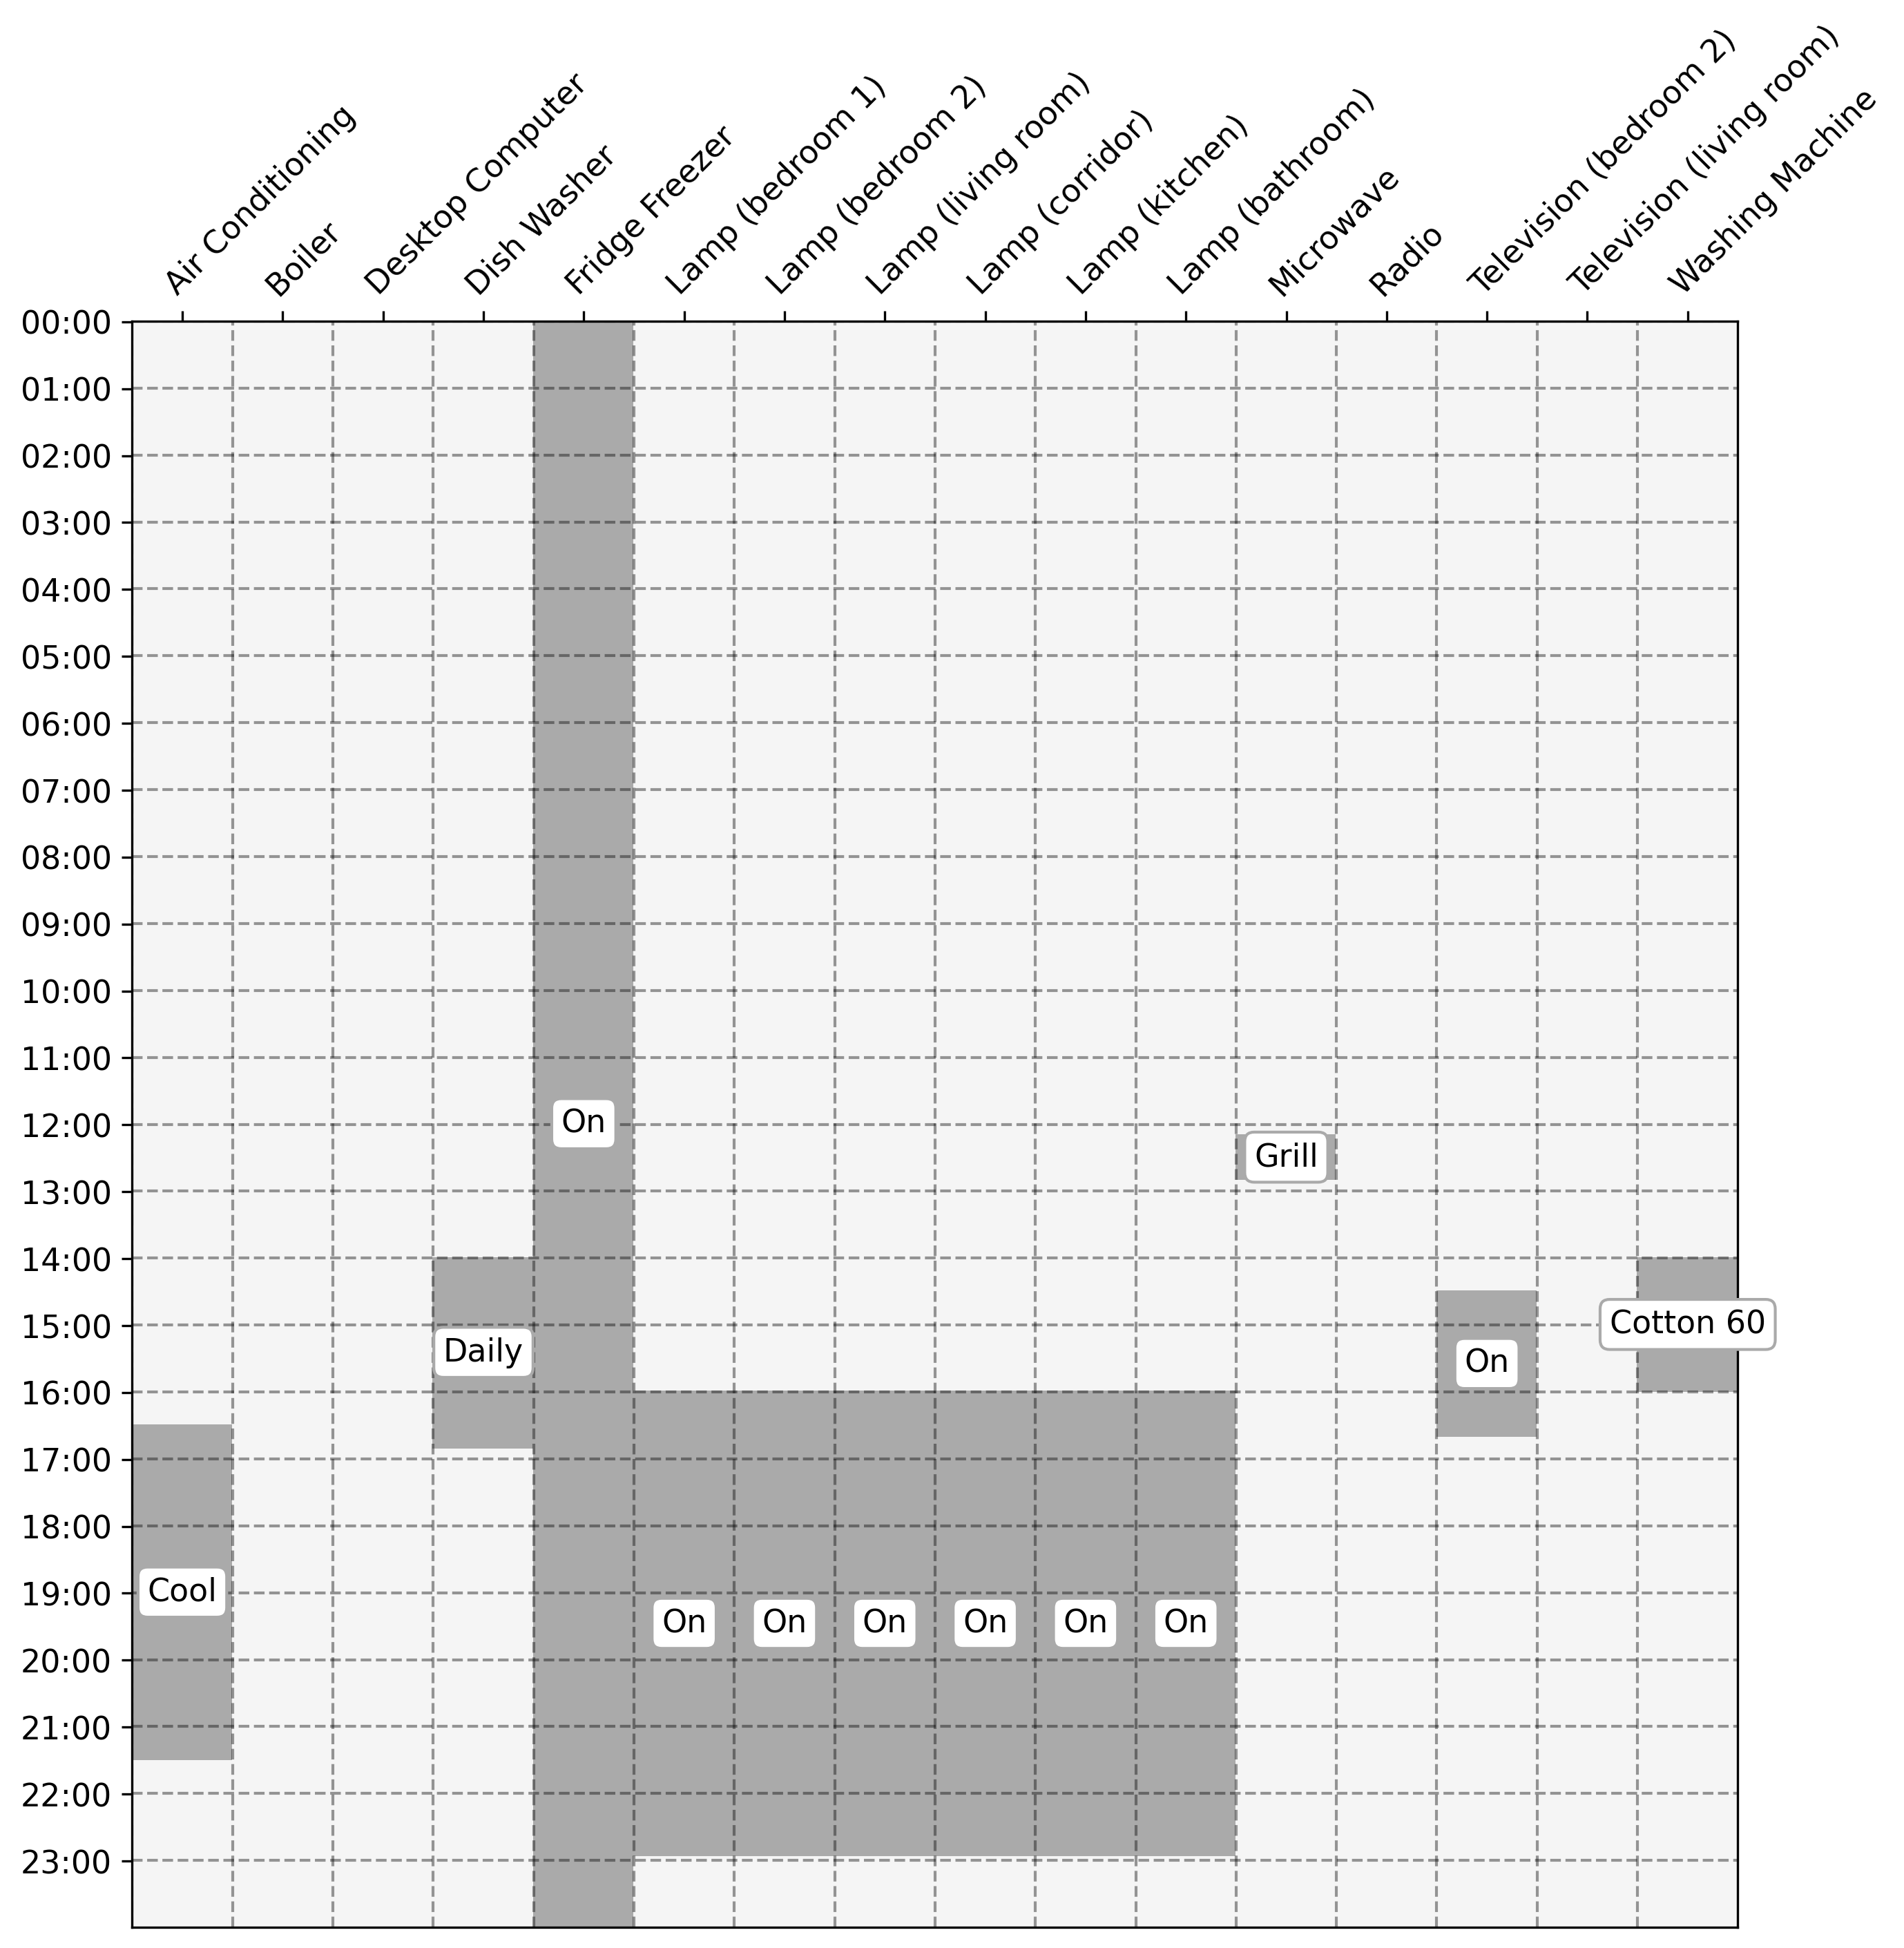
\includegraphics[width=0.9\textwidth]{images/real_matrix.png}
    \caption{Consumptions matrix of registered routines}
    \label{fig:existing_consumption_matrix}
\end{figure}

\begin{figure}
    \centering
    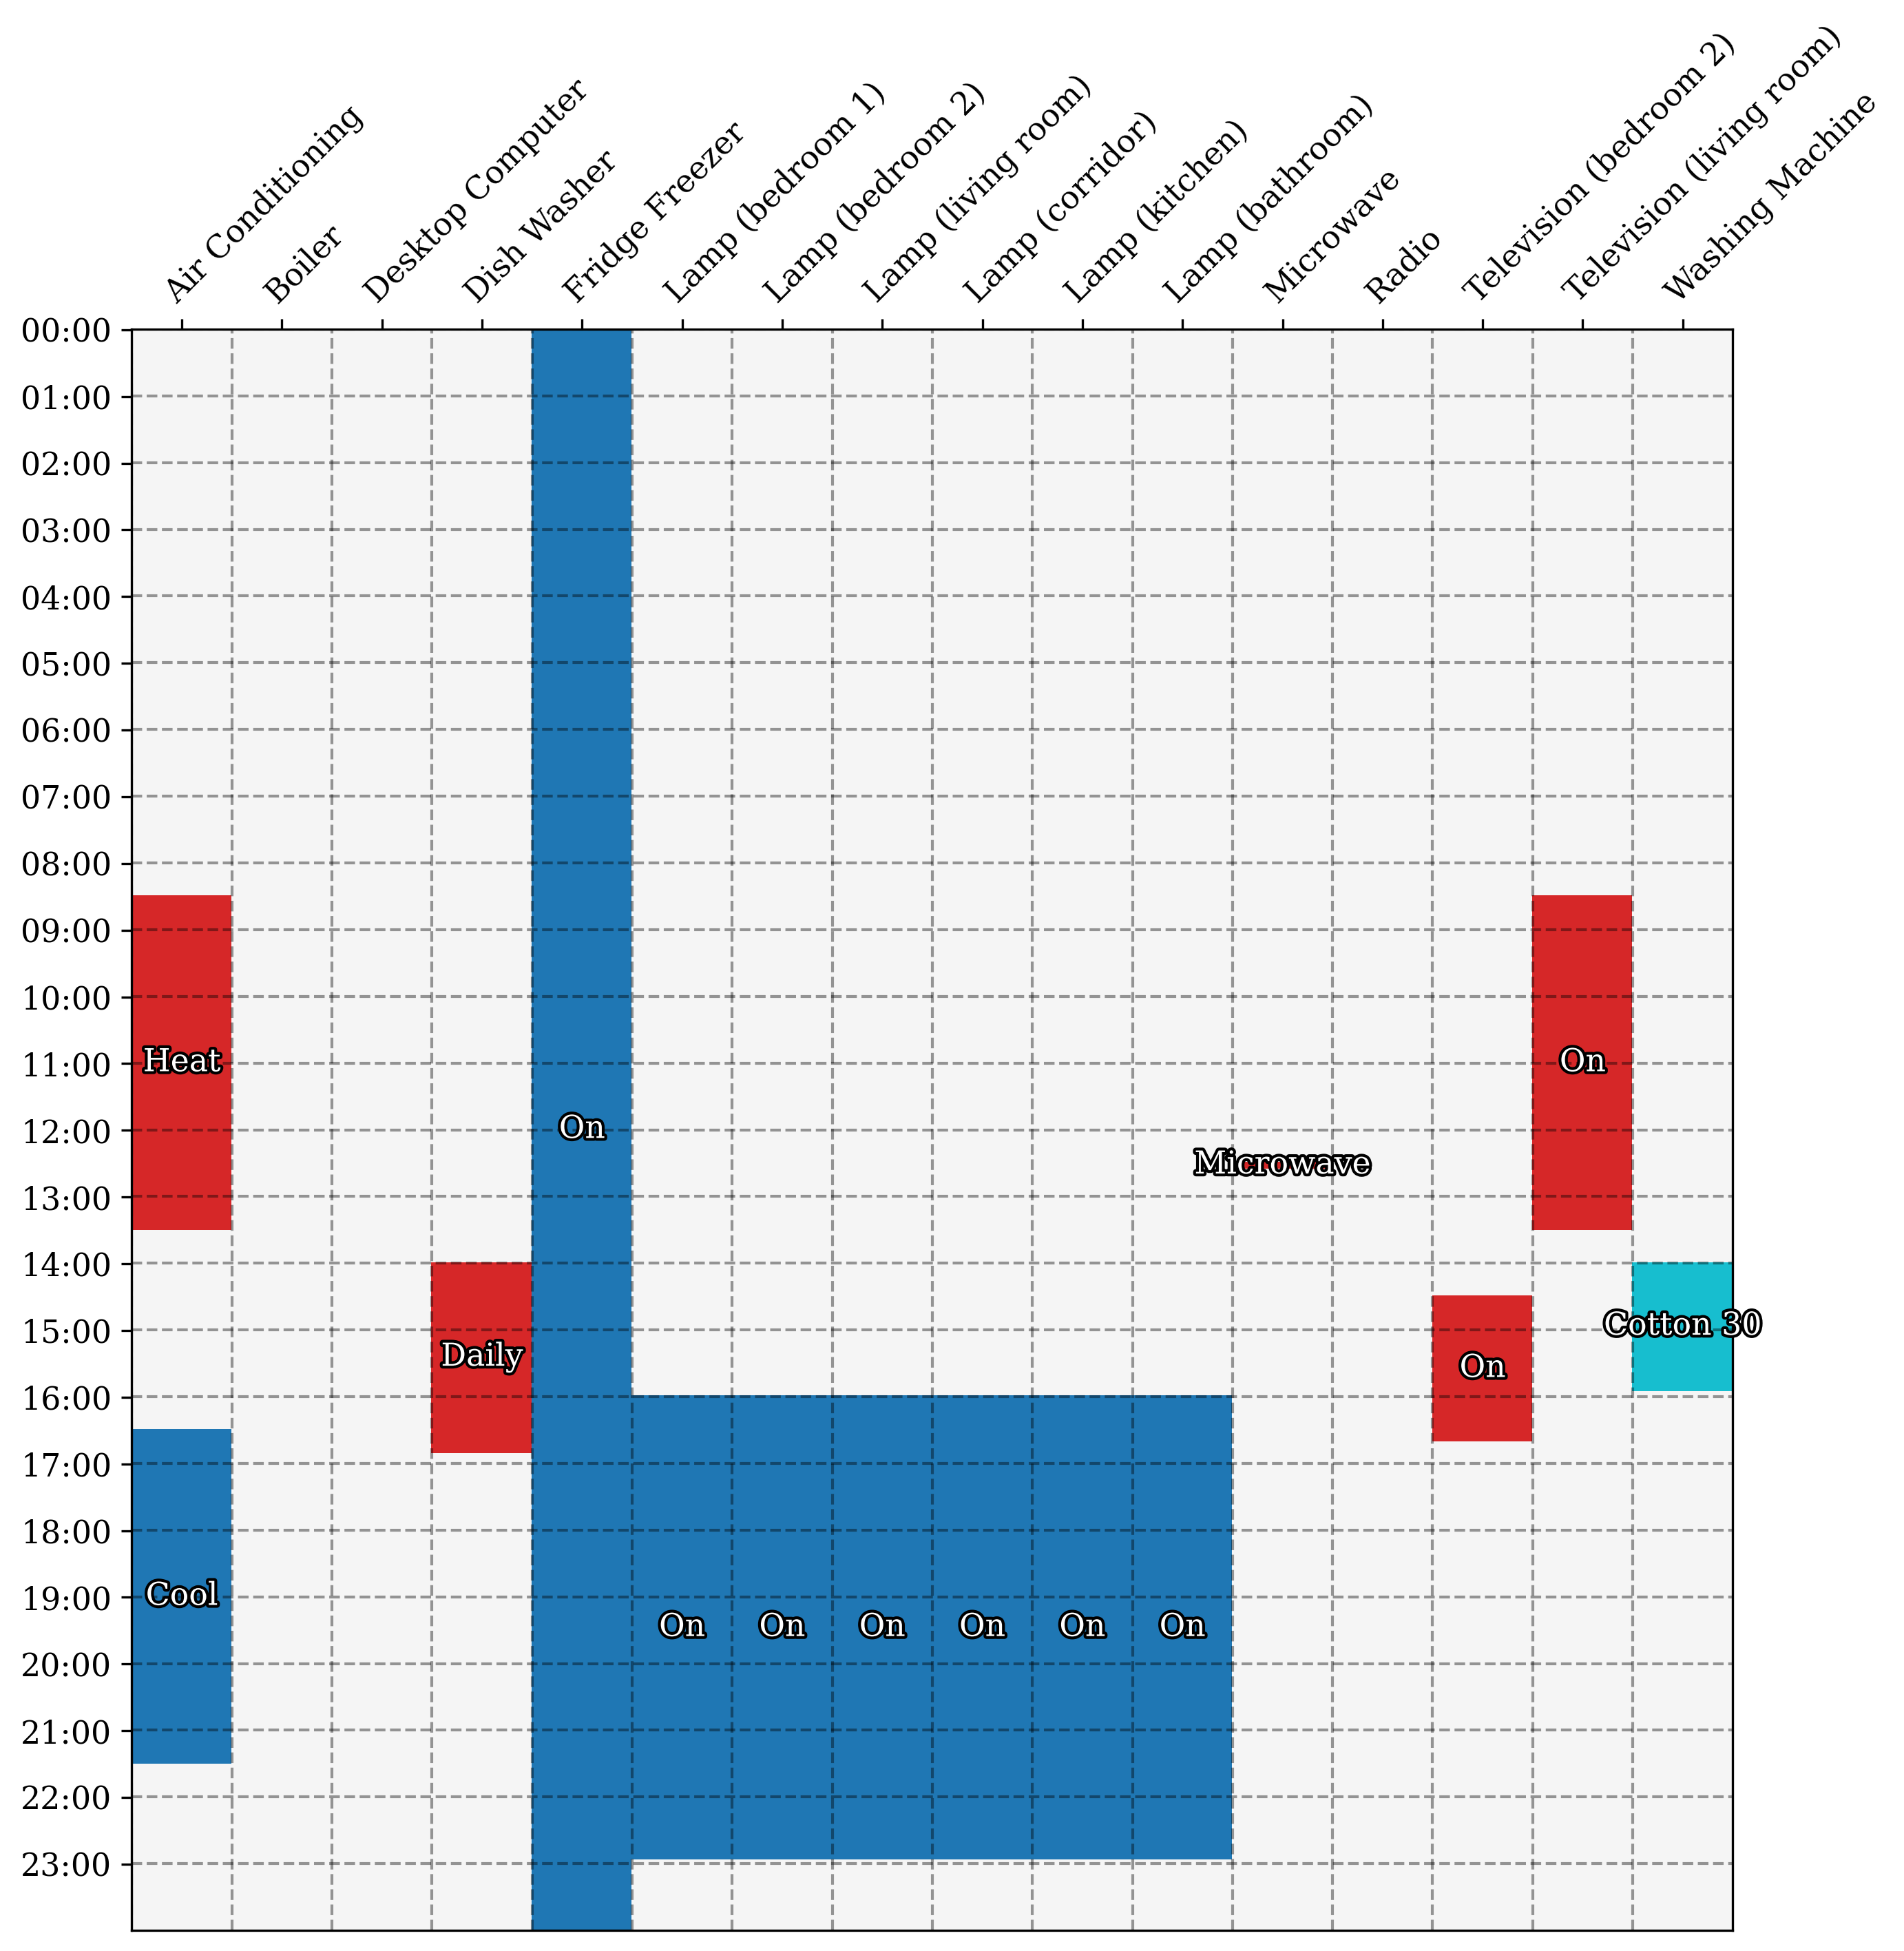
\includegraphics[width=0.9\textwidth]{images/simulated_matrix.png}
    \caption{Simulated matrix.}
    \label{fig:simulated_consumption_matrix}
\end{figure}

\section{REST API}